\documentclass[10pt]{article}
\usepackage{array, xcolor, lipsum, bibentry}
\usepackage[a4paper, top=2cm, bottom=2cm]{geometry}


\usepackage{multirow}


\usepackage[T1]{fontenc}	      
\usepackage[english]{babel}
\usepackage[utf8]{inputenc}
\usepackage{graphicx}

\usepackage{libertine}
\usepackage{hyperref}
\hypersetup{
colorlinks=true
}

\title{Kristofer Leifland}
\author{}
\date{}
\definecolor{lightgray}{gray}{0.8}
\newcolumntype{L}{>{\raggedleft}p{0.14\textwidth}}
\newcolumntype{R}{p{0.8\textwidth}}
\newcommand\VRule{\color{lightgray}\vrule width 0.5pt}
\begin{document}
\maketitle
\thispagestyle{empty}
\pagestyle{empty}
\noindent



\noindent
Kristofer Leifland <\href{mailto:kristofer.leifland@gmail.com}{\nolinkurl{kristofer.leifland@gmail.com}}>\\
Barometergatan 58, 211 17 Malmö\\
+46 (0)722 110494\\

%\begin{figure}[ht!]
%\centering
%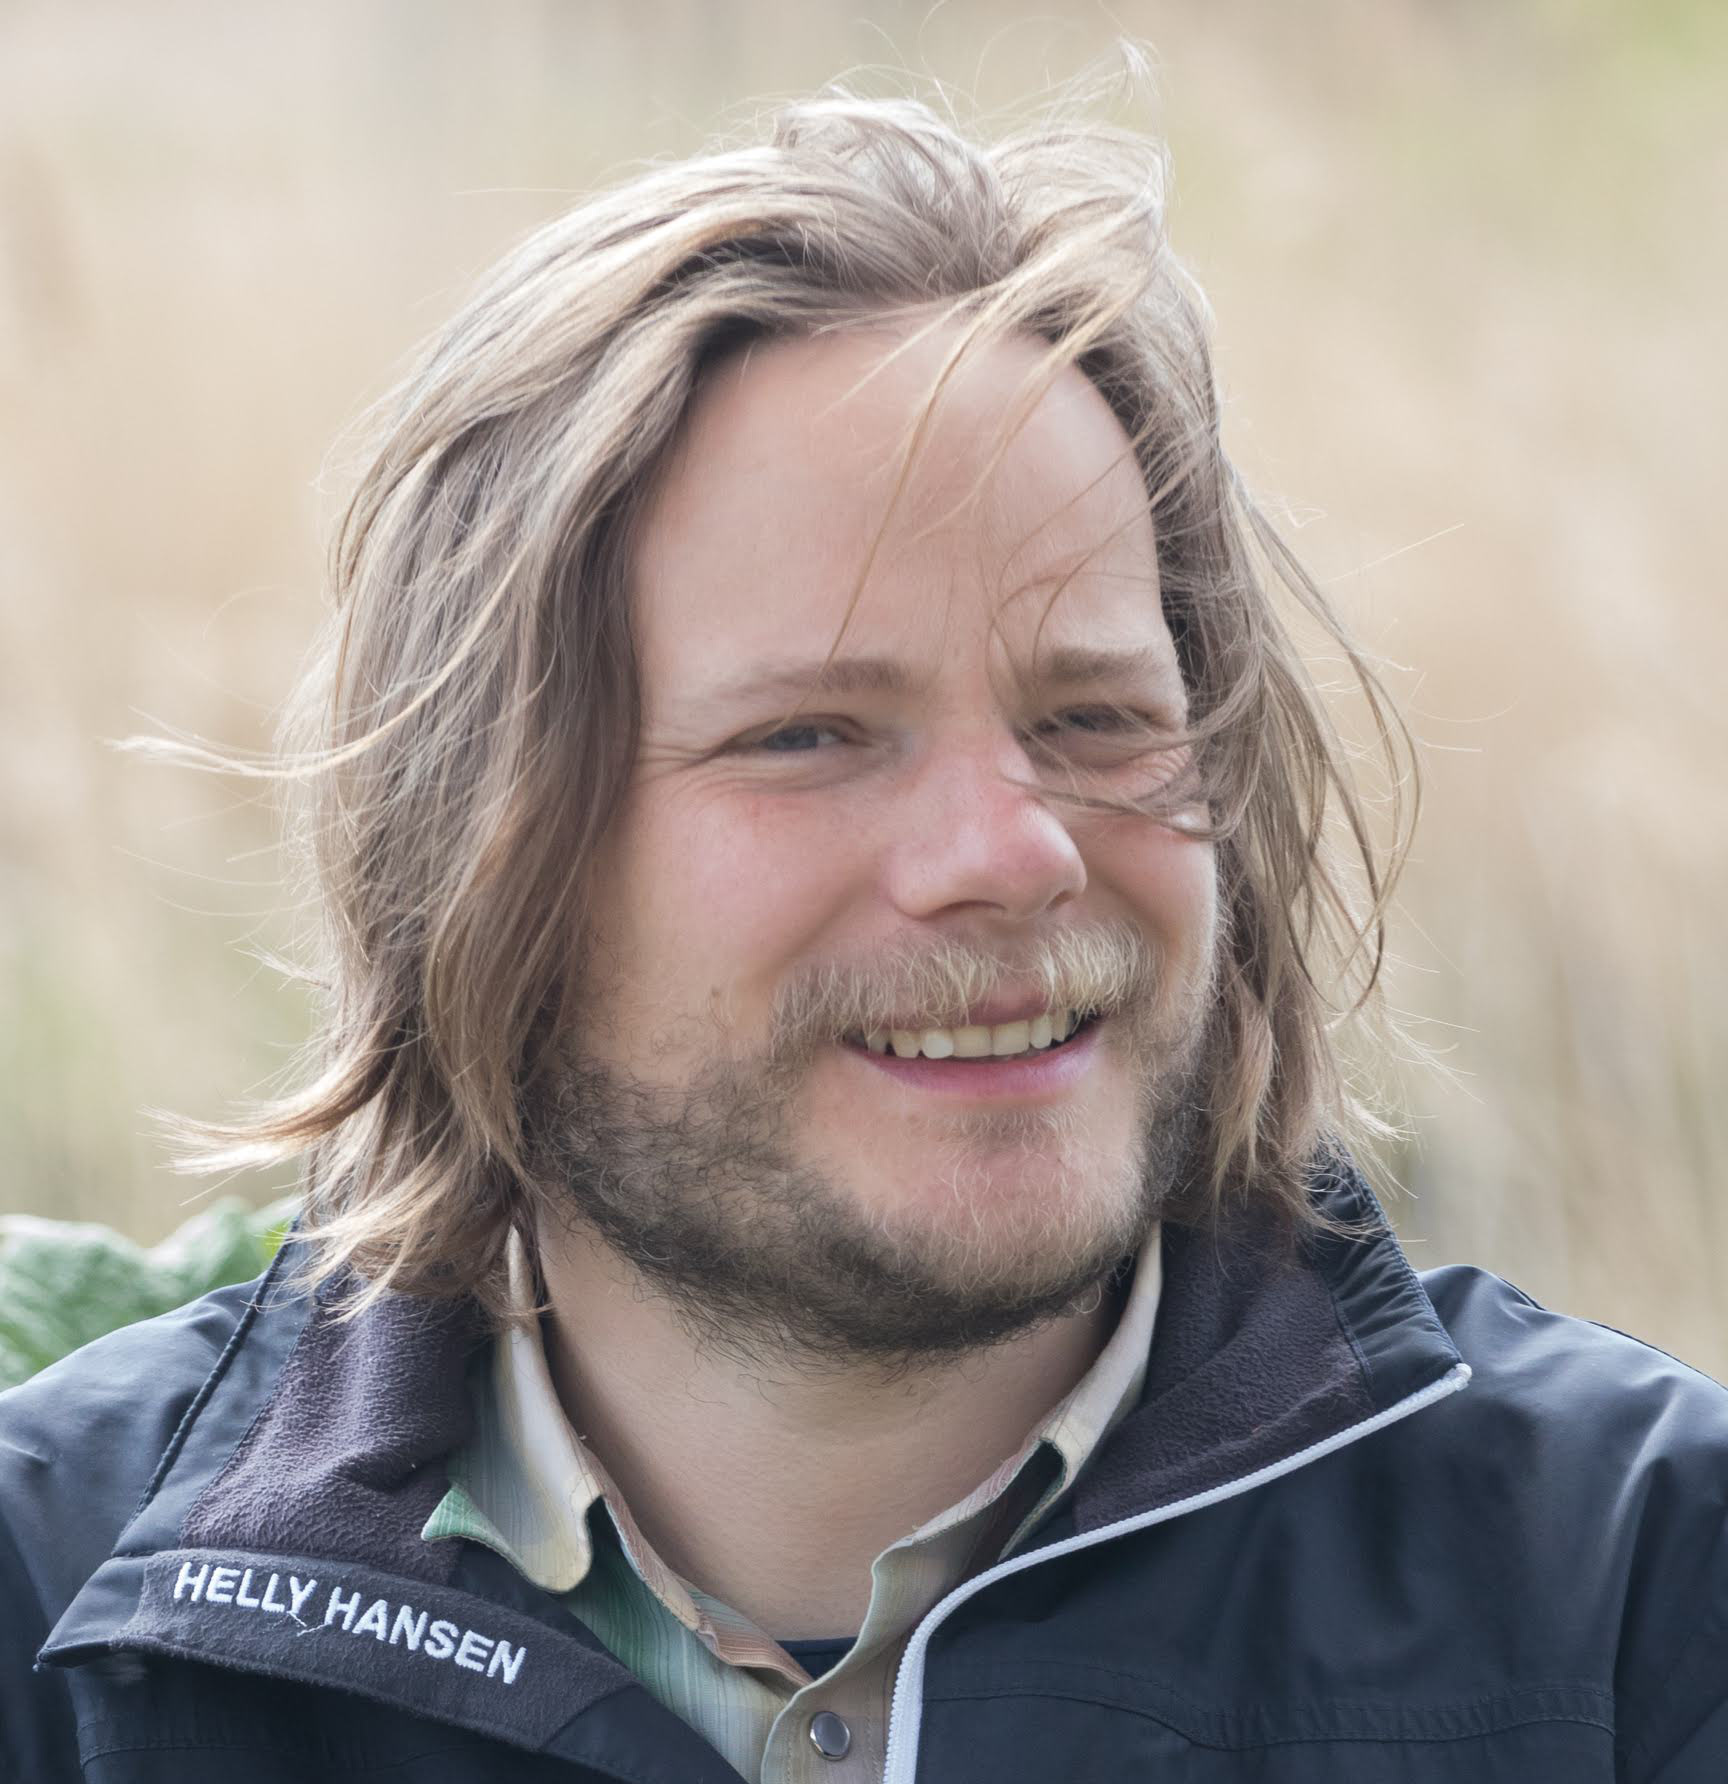
\includegraphics[width=20mm]{me.jpg}
%\end{figure}
%\begin{minipage}[ht]{0.48\textwidth}
%January 3rd, 2020\\
%+12 34 56 789
%\end{minipage}

\section*{Objective}
Keep improving as a software craftsman. Find people and environments that provide good fellowship and meaningful outputs.

\section*{Experience}
\begin{tabular}{L!{\VRule}R}
2014--now&{\bf Software Engineer at AFRY}\\
&Software development consultant with focus on Scala and Java. Assignments include:

\begin{itemize}
  \item Developing Scala/Java backend services and Spark pipelines for a well known global maps service. Current assignment, since 2015.
  \item Writing public API backend endpoints in Java for a Swedish bank.
  \item Making the Android application for an automated animal feeding device.
  \item Implementing new features in a gas station inspection application.
  \item Adding invoice integration for an e-commerce application.
\end{itemize}
\\
Spring 2014&{\bf Thesis Work at ÅF AB}\\
&We developed a system that uses crowdsourcing and gamification to map urban sound environments using smartphones.\\
2012--2014&{\bf Computer Science Lab Assistant at Malmö University}\\
&Graded student assignments and assisted during computer science lab work.\\
Fall 2012&{\bf Support Function at Syngenta Seeds AB}\\
&Various tasks related to a software migration project. Development of a seed quality report in QlikView, migration of an Access database, writing Excel VBA scripts, and more.\\
Summer 2012&{\bf Web Developer Intern at 23 Gears}\\
&I developed a web application that allows users to browse and create new issues using a custom interface to Jira.\\
2010--2012&{\bf Product Evaluation Assistant at Syngenta Seeds AB}\\
&My routine tasks included data management and assisting in trial planning within the PE group. I was also deeply involved in various statistical projects within the plant breeding group.\\
\end{tabular}

\section*{Education}
\begin{tabular}{L!{\VRule}R}
2011--2014 & {\bf Bachelor of Science in Engineering, Computer Engineering, Malmö University}\\
&Focus on courses in computer science. \\
2002--2008&{\bf Degree of Master of Science in Environmental Science, Lund University}\\
&In my thesis work I evaluated several biomass models for crayfish stock assessments, see \url{http://goo.gl/DtSNY}. \\
%\vspace{5pt}\\
\end{tabular}

%\section*{Languages}
%\begin{tabular}{L!{\VRule}R}
%Swedish&Mother tongue\\
%English&Fluent\\
%French&Some\\
%\end{tabular}

\end{document}
